%!TEX ROOT=../ctutest.tex

\chapter{Current Contribution}
\label{chap:contribution}

\textit{We have collected novel data for the fact-checking task in our application context, emulated and scraped inavailable datasets making them public or readying them for doing so, we have established numerous state-of-the-art models and we are currently working on establishing the topic of claim generation as a summarization-related NLP task.}

\section{Datasets}
Having the automated fact-checking scheme established in chapter~\ref{chap:sota}, every machine-learning solution must start with the choice or collection of appropriate training data.
Due to the novelty of the task in Czech and other West Slavic languages, I explored a multitude of ways to acquire such data, many of them resulting in a publicly available dataset in our Huggingface repository~\footnote{\url{https://huggingface.co/ctu-aic}}, beginning to be reused by others. 

\subsection{\FCZ}\label{sec:fcz}
An early \"{temporary benchmark} for our endeavours in adapting the FEVER~\cite{fever} task for the Czech context was the \FCZ~\cite{lrev} dataset.

In~\cite{diplomka}, I have proposed a simple FEVER data transduction scheme that can be simplified as follows:

\begin{enumerate}
    \item Each FEVER claim is translated using the (at the time maturing) Machine Translator
    \item Evidence from English Wikipedia is not translated using MT, but mapped onto its Czech-Wikipedia counterpart using the publicly available Wikidata\footnote{Used, for example, for showing the \"{see this article in other languages} suggestions in Wikipedia sidebar}
    \item Data with any loss in evidence due to the step 2. is discarded
\end{enumerate}

This design was relatively cheap to compute (as translating the whole 2017 Wikipedia corpus would have been a long and wasteful computation), delivering an open-license dataset of 127K claims, their labels and evidence justifications. My hope was, as both the 2017 EnWiki and our 2020 CsWiki corpus only featured the first paragraph (abstract) of each article, a document-level alignment could be assumed -- both the Czech and English text always summarize the basic facts about the same entity.

This showed to be only partly true as a later human annotation on a 1\% sample of \FCZ data showed that about a third of data exhibits some levels of noise, mostly introduced during dataset translation~\cite{lrev}.

While noisy, the \FCZ data still got its use in training of the information retrieval schemes of~\cite{rypar,gazo,lrev} used to this day and is openly available\footnote{\url{https://huggingface.co/datasets/ctu-aic/csfever}} under a CC license.

My research on it also motivated a creation of a inference-only version of the dataset, which does not support the Information Retrieval task and therefore, does not require the mapping of evidence into a live version of Wikipedia.
Therefore, only the EnWiki \textit{excerpts} needed to build evidence can be translated, bringing down the computational difficulty and enabling me to deliver a dataset without the transduction noise called \FCZNLI\footnote{\url{https://huggingface.co/datasets/ctu-aic/csfever_nli}}. 

Another round of research \FCZ motivated and I supervised was the successful thesis of~\cite{mlynar}, modernizing the data and machine-translation methods into the 2023 state of the art.
\cite{mlynar} further experimented with methods of automated noise detection and removal, which has not shown to be an efficient way to tackle the issue of high noise in \FCZ.

However, it delivers a partly cleaned versions of it\footnote{\url{https://huggingface.co/datasets/ctu-aic/csfever_v2}} and motivates a future research of generating such data differently, using a claim generation scheme like that from~\cite{pan2021zeroshot}.


\subsection{FCheck Annotations Platform}
The imperfections in translated \FCZ data, as well as the ongoing colaboration with ČTK and the Faculty of Social Sciences brought me to also look for ways how to hand-annotate a whole new natively Czech dataset, which would both lack the noise of translated data and take the task of automated fact checking to next level, replacing a rigid, simple Wikipedic data with a more \"{real world} news report corpus of ČTK.

Figure~\ref{fig:fcheck} shows an open-source platform FCheck\footnote{\url{https://fcheck.fel.cvut.cz} (\texttt{testuser}), source at: \href{https://github.com/aic-factcheck/fcheck-annotations-platform}{\texttt{github.com/aic-factcheck/fcheck-annotations-platform}}} I developed to collaborate with 316 FSV CUNI students of on a collection of novel dataset in Czech using ČTK data as a ground truth corpus.
\label{sec:datasets}
\begin{figure}[H]
    \makebox[\textwidth][c]{
    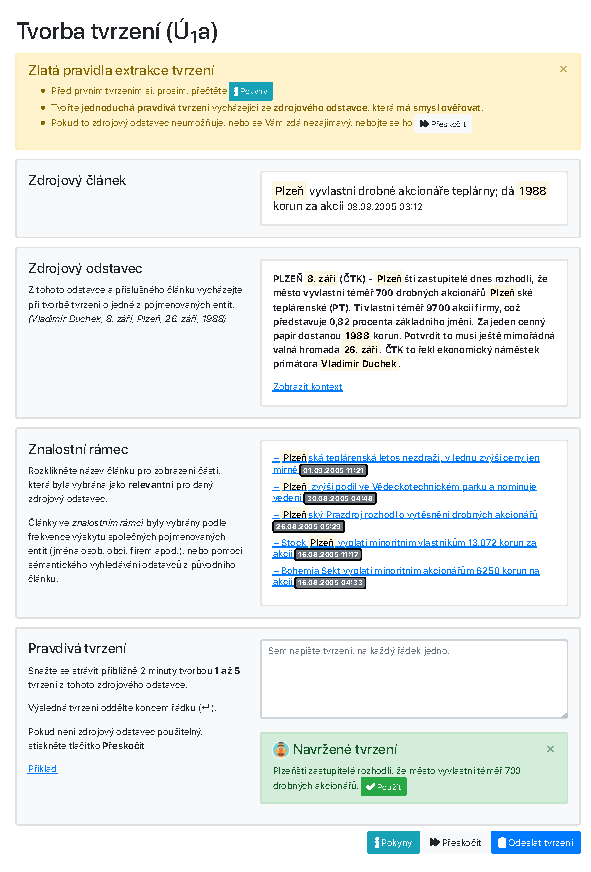
\includegraphics[height=7.5cm]{fig/fcheck/claim_extraction.pdf}
    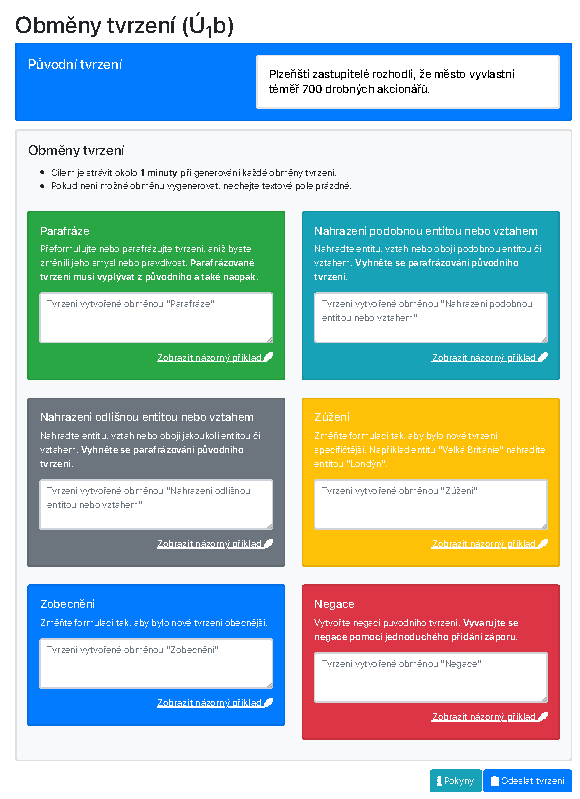
\includegraphics[height=7.5cm]{fig/fcheck/mutation.pdf}
    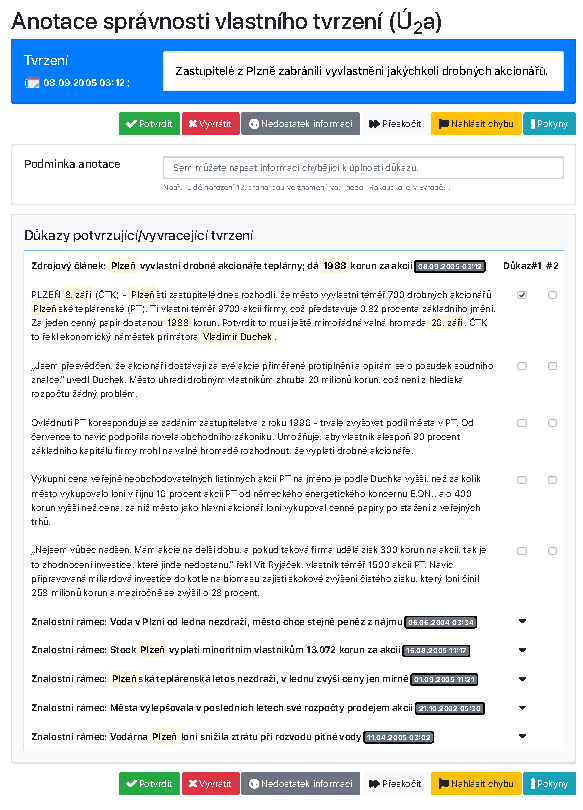
\includegraphics[height=7.5cm]{fig/fcheck/annotation.pdf}
    }
    \caption{{\techbf FCheck} -- platform for fact-checking data collection developed for TAČR project; collects data for claim generation, information retrieval and natural language inference tasks}
    \label{fig:fcheck}
\end{figure}

We have established a 4-step annotation procedure inspired by the time-proven methodology of~\cite{fever} where chech-worthy paragraphs are first hand-picked among samples from the whole archive of ČTK's 3.3 M news reports published between 1 January 2000 and 6 March 2019. Then, the annotator is sampled such a paragraph and asked to \textit{extract claims} from it, i.e., formulate single-sentence summaries of some facts that appear in paragraph. This claim is always \textit{supported} by the data, so the next phase is to perturb the claim by annotator's world knowledge and form the claim \textit{mutations} -- substitutions of entities, generalizations, specifications, paraphrases or negations of the original claim. 
The mutated claim is then fact-checked by (typically) another annotator, using the ČTK data narrowed down to a reasonable number of relevant articles (in an IR sense) as \textit{supportable}, \textit{refutable} or \textit{not enough info}, providing a set of evidence as a verdict justification.

The whole application is running on multiple levels -- a yii-framework-powered PHP app is running the annotation interface, while a flask server in python is running our models based on TF-IDF~\cite{drqa} and mBERT (section~\ref{sec:bert}) for information retrieval trained among other data on the \FCZ dataset (section~\ref{sec:fcz}).
The models are solving the Information Retrieval task on-demand (with cache) on the proprietary ČTK corpus, whenever the annotation app needs it to provide a context to the fact-checker.

The scheme and its implementations are exhaustively described in~\cite{diplomka}, chapter 4 and in~\cite{lrev}, also chapter 4.
Multiple \"{cross-annotations} were collected for each claim, to measure agreement and give insights into task complexity.

\subsection{\CTK}
\label{sec:ctkfacts}

\begin{table}
    \begin{center}
        \begin{minipage}{\textwidth}
            \caption{Label distribution in \CTK splits before and after cleaning. Reprinted from~\cite{lrev}}\label{tab:ctkfacts-overview}
            \begin{tabular*}{\textwidth}{@{\extracolsep{\fill}}lllllll@{\extracolsep{\fill}}}
                \toprule
                & \multicolumn{3}{@{}c@{}}{\CTK uncleaned, balanced} & \multicolumn{3}{@{}c@{}}{\CTK cleaned, stratified}\\
                \cmidrule{2-4}\cmidrule{5-7}
                Split & {\texttt{SUPPORTS}} & \texttt{REFUTES}  & \texttt{NEI} & {\texttt{SUPPORTS}} & \texttt{REFUTES}  & \texttt{NEI}\\
                \midrule
                \train  & 1,164 & 549 & 503     & 1,104 & 556 & 723 \\
                \dev    & 100 & 100 & 100       & 142 & 85 & 105\\
                \test   & 200 & 200 & 200       & 176 & 79 & 127\\
                \botrule
            \end{tabular*}
        \end{minipage}
    \end{center}
\end{table}

After completing the first year annotation runs, we have extracted a total of 3,116 multi-annotated claims.
47\% were \texttt{SUPPORT}ed by the majority of their annotations, \REF{} and \NEI{} labels were approximately even, the full distribution of labels is listed in Table~\ref{tab:ctkfacts-overview}.
% We have originally experimented with balanced \dev and \test splits to punish predictors exploiting this bias.

Of all the annotated claims, 1,776, that is 57\%, had at least two independent labels assigned by different annotators.
This sample was given by the intrinsic randomness of mutated claim sampling.
In this section, we use it to asses the quality of our data and ambiguity of the task, as well as to propose annotation cleaning methods used to arrive to our final \text{cleaned} \CTK dataset.

\subsubsection{Inter-Annotator Agreement}
\label{sec:agreement}

Due to our cross-annotation design, I had generously sized sample of independently annotated labels in our hands.
As the total number of annotators was greater than 2, and as we allowed missing observations, we have used the Krippendorff's alpha measure~\cite{krippendorff1970} which is the standard for this case~\cite{hayes2007krippendorff}.
For the comparison with \cite{fever} and \cite{norregaard2021danfever}, we also list a 4-way Fleiss' $\kappa$-agreement~\cite{fleiss1971measuring} calculated on a sample of 7.5\% claims.

We have calculated the resulting Krippendorff's alpha agreement to be 56.42\% and Fleiss' $\kappa$ to be 63\%.
We interpret this as an adequate result that testifies to the complexity of the task of news-based fact verification within a fixed knowledge scope.
It also encourages a round of annotation cleaning experiments that would exploit the number of cross-annotated claims to remove common types of noise.

\subsection{Other NLP datasets in West Slavic languages}
\begin{enumerate}
    \item {\techbf Translated NLI datasets} -- SNLI, ANLI, MultiNLI, 
    \item SmeSum, CTKSum, CsFEVERSum
    \item Polish summarization data
\end{enumerate}
\section{Models}
\label{sec:models}
\section{Publications}
\label{sec:publications}
\section{Applications}
\label{sec:applications}

\begin{figure}
    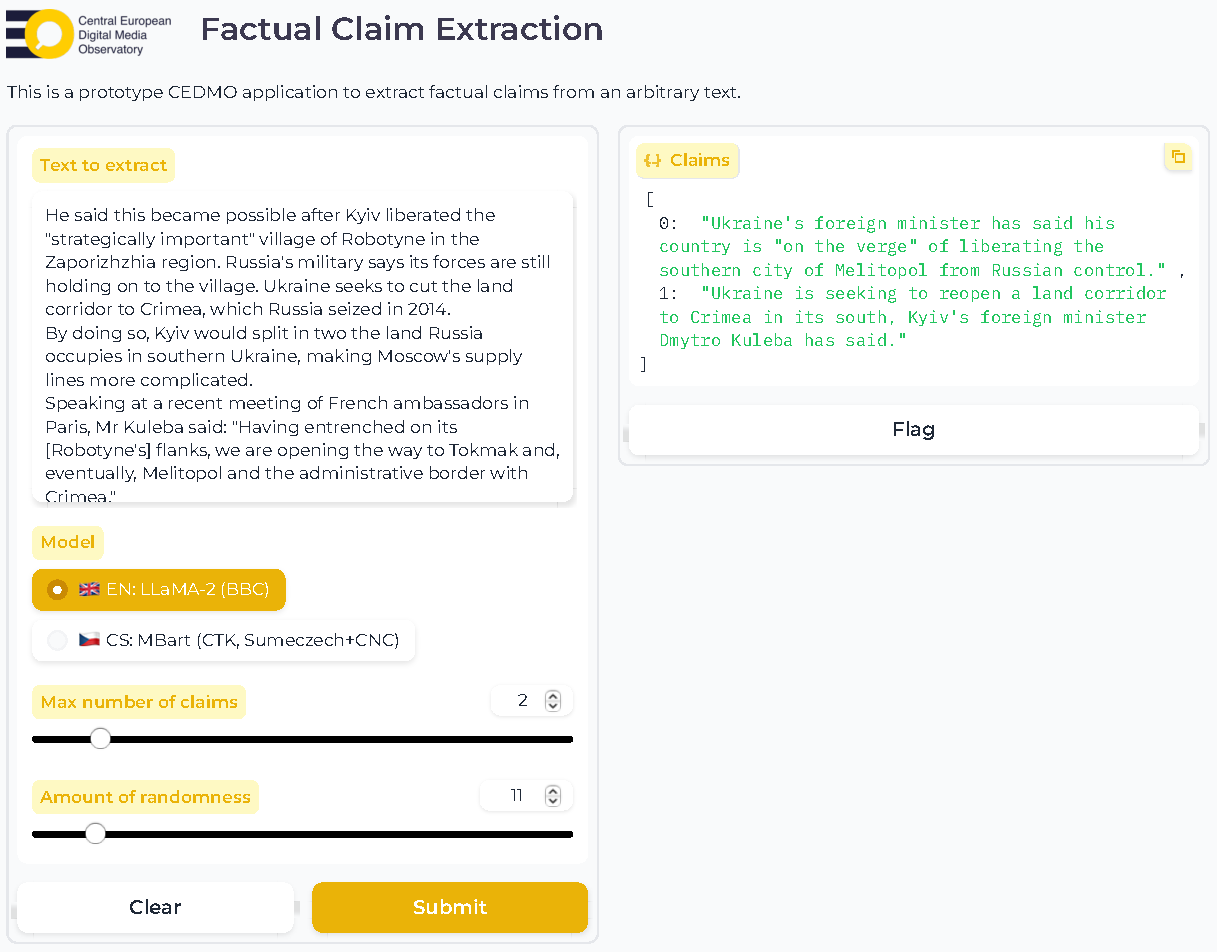
\includegraphics[width=16cm]{fig/cedmo.pdf}
    \caption{Factual claim extraction application done for the CEDMO project}
    \label{fig:framework}
\end{figure}

Here we will show off the demonstration tools, as well as our open-source platform \url{https://fcheck.fel.cvut.cz} and currently running claim extraction tools. 